\documentclass[11pt,a4paper]{article}

% ----- preamble.tex -----
% % ----- preamble.tex -----
% % ----- preamble.tex -----
% \input{preamble.tex} should be included in all note files before '\begin{document}'
% \lecture{<lectureNumber>: <lectureTopic>}{<mm/dd/yyyy>}{<lecturerName>}{<authorName>}

\hbadness=10000
\vbadness=10000

% page size settings
\setlength{\textheight}{8.5in}
\setlength{\textwidth}{6.0in}
\setlength{\headheight}{0in}
\addtolength{\topmargin}{-.5in}
\addtolength{\oddsidemargin}{-.5in}

% paragraph spacing/indenting settings
\setlength\parindent{0pt}
\setlength\parskip{2.5pt}

% imported packages
\usepackage{amsmath,amssymb,amsthm}
\usepackage{mdframed} % for boxing
\usepackage{graphicx} % for inserting images
\graphicspath{ {./imgs/} }

\usepackage{diagbox} % backslash for tabular/tables
\usepackage{booktabs} % enhances quality of table presentation
\usepackage{tikz}
\usetikzlibrary{arrows,automata,trees,calc}

% ----- \tableofcontents PAGE LINKING (without blue highlight) -----
\usepackage{hyperref}
\hypersetup{
    colorlinks,
    citecolor=black,
    filecolor=black,
    linkcolor=black,
    urlcolor=black
}

% ----- VARIABLE RE-DEFINITIONS -----
\def\epsilon{\varepsilon}
\def\phi{\varphi}


% ----- TODO: MAKE EVERY NEW SECTION START ON NEW PAGE EXCLUDING TOC -----
% \let\oldsection\section
% \renewcommand{\section}{\newpage\oldsection}


% ----- CUSTOM COMMANDS -----
\newcommand{\handout}[5]{
    % \renewcommand{\thepage}{#1-\arabic{page}}
    \noindent
    \begin{center}
        \framebox{
            \vbox{
                \hbox to 5.78in {{\bf CS 4510: Automata and Complexity}\hfill #2}
                \vspace{4mm}
                \hbox to 5.78in {{\Large \hfill #5  \hfill}}
                \vspace{2mm}
                \hbox to 5.78in {{\it #3 \hfill #4}}
            }
        }
   \end{center}
   \vspace*{4mm}
}

\newcommand{\lecture}[4]{\handout{#1}{#2}{Lecturer: #3}{Author: #4}{Lecture #1}}

% keeps contents of the same theorem on the same page
\newcommand{\blocktheorem}[1]{
    \csletcs{old#1}{#1}
    \csletcs{endold#1}{end#1}
    \RenewDocumentEnvironment{#1}{o}{
        % \par\addvspace{cm}
        \noindent\begin{minipage}{\textwidth}
        \IfNoValueTF{##1}{\csuse{old#1}}{\csuse{old#1}[##1]}}{\csuse{endold#1}
        \end{minipage}
        \par\addvspace{0.75cm}
    }
}
\raggedbottom

\theoremstyle{definition}
\newtheorem{example}{Example} % use for example problems
\newmdtheoremenv{definition}{Definition} % use for definitions
\newtheorem{theorem}{Theorem} % use for theorems
\newtheorem{corollary}{Corollary} % use for corollary
\newtheorem{lemma}{Lemma} % use for corollary
\newtheorem{claim}{Claim}

\blocktheorem{example}
\blocktheorem{definition}
\blocktheorem{theorem}
\blocktheorem{corollary}
\blocktheorem{lemma}
\blocktheorem{claim} should be included in all note files before '\begin{document}'
% \lecture{<lectureNumber>: <lectureTopic>}{<mm/dd/yyyy>}{<lecturerName>}{<authorName>}

\hbadness=10000
\vbadness=10000

% page size settings
\setlength{\textheight}{8.5in}
\setlength{\textwidth}{6.0in}
\setlength{\headheight}{0in}
\addtolength{\topmargin}{-.5in}
\addtolength{\oddsidemargin}{-.5in}

% paragraph spacing/indenting settings
\setlength\parindent{0pt}
\setlength\parskip{2.5pt}

% imported packages
\usepackage{amsmath,amssymb,amsthm}
\usepackage{mdframed} % for boxing
\usepackage{graphicx} % for inserting images
\graphicspath{ {./imgs/} }

\usepackage{diagbox} % backslash for tabular/tables
\usepackage{booktabs} % enhances quality of table presentation
\usepackage{tikz}
\usetikzlibrary{arrows,automata,trees,calc}

% ----- \tableofcontents PAGE LINKING (without blue highlight) -----
\usepackage{hyperref}
\hypersetup{
    colorlinks,
    citecolor=black,
    filecolor=black,
    linkcolor=black,
    urlcolor=black
}

% ----- VARIABLE RE-DEFINITIONS -----
\def\epsilon{\varepsilon}
\def\phi{\varphi}


% ----- TODO: MAKE EVERY NEW SECTION START ON NEW PAGE EXCLUDING TOC -----
% \let\oldsection\section
% \renewcommand{\section}{\newpage\oldsection}


% ----- CUSTOM COMMANDS -----
\newcommand{\handout}[5]{
    % \renewcommand{\thepage}{#1-\arabic{page}}
    \noindent
    \begin{center}
        \framebox{
            \vbox{
                \hbox to 5.78in {{\bf CS 4510: Automata and Complexity}\hfill #2}
                \vspace{4mm}
                \hbox to 5.78in {{\Large \hfill #5  \hfill}}
                \vspace{2mm}
                \hbox to 5.78in {{\it #3 \hfill #4}}
            }
        }
   \end{center}
   \vspace*{4mm}
}

\newcommand{\lecture}[4]{\handout{#1}{#2}{Lecturer: #3}{Author: #4}{Lecture #1}}

% keeps contents of the same theorem on the same page
\newcommand{\blocktheorem}[1]{
    \csletcs{old#1}{#1}
    \csletcs{endold#1}{end#1}
    \RenewDocumentEnvironment{#1}{o}{
        % \par\addvspace{cm}
        \noindent\begin{minipage}{\textwidth}
        \IfNoValueTF{##1}{\csuse{old#1}}{\csuse{old#1}[##1]}}{\csuse{endold#1}
        \end{minipage}
        \par\addvspace{0.75cm}
    }
}
\raggedbottom

\theoremstyle{definition}
\newtheorem{example}{Example} % use for example problems
\newmdtheoremenv{definition}{Definition} % use for definitions
\newtheorem{theorem}{Theorem} % use for theorems
\newtheorem{corollary}{Corollary} % use for corollary
\newtheorem{lemma}{Lemma} % use for corollary
\newtheorem{claim}{Claim}

\blocktheorem{example}
\blocktheorem{definition}
\blocktheorem{theorem}
\blocktheorem{corollary}
\blocktheorem{lemma}
\blocktheorem{claim} should be included in all note files before '\begin{document}'
% \lecture{<lectureNumber>: <lectureTopic>}{<mm/dd/yyyy>}{<lecturerName>}{<authorName>}

\hbadness=10000
\vbadness=10000

% page size settings
\setlength{\textheight}{8.5in}
\setlength{\textwidth}{6.0in}
\setlength{\headheight}{0in}
\addtolength{\topmargin}{-.5in}
\addtolength{\oddsidemargin}{-.5in}

% paragraph spacing/indenting settings
\setlength\parindent{0pt}
\setlength\parskip{2.5pt}

% imported packages
\usepackage{amsmath,amssymb,amsthm}
\usepackage{mdframed} % for boxing
\usepackage{graphicx} % for inserting images
\graphicspath{ {./imgs/} }

\usepackage{diagbox} % backslash for tabular/tables
\usepackage{booktabs} % enhances quality of table presentation
\usepackage{tikz}
\usetikzlibrary{arrows,automata,trees,calc}

% ----- \tableofcontents PAGE LINKING (without blue highlight) -----
\usepackage{hyperref}
\hypersetup{
    colorlinks,
    citecolor=black,
    filecolor=black,
    linkcolor=black,
    urlcolor=black
}

% ----- VARIABLE RE-DEFINITIONS -----
\def\epsilon{\varepsilon}
\def\phi{\varphi}


% ----- TODO: MAKE EVERY NEW SECTION START ON NEW PAGE EXCLUDING TOC -----
% \let\oldsection\section
% \renewcommand{\section}{\newpage\oldsection}


% ----- CUSTOM COMMANDS -----
\newcommand{\handout}[5]{
    % \renewcommand{\thepage}{#1-\arabic{page}}
    \noindent
    \begin{center}
        \framebox{
            \vbox{
                \hbox to 5.78in {{\bf CS 4510: Automata and Complexity}\hfill #2}
                \vspace{4mm}
                \hbox to 5.78in {{\Large \hfill #5  \hfill}}
                \vspace{2mm}
                \hbox to 5.78in {{\it #3 \hfill #4}}
            }
        }
   \end{center}
   \vspace*{4mm}
}

\newcommand{\lecture}[4]{\handout{#1}{#2}{Lecturer: #3}{Author: #4}{Lecture #1}}

% keeps contents of the same theorem on the same page
\newcommand{\blocktheorem}[1]{
    \csletcs{old#1}{#1}
    \csletcs{endold#1}{end#1}
    \RenewDocumentEnvironment{#1}{o}{
        % \par\addvspace{cm}
        \noindent\begin{minipage}{\textwidth}
        \IfNoValueTF{##1}{\csuse{old#1}}{\csuse{old#1}[##1]}}{\csuse{endold#1}
        \end{minipage}
        \par\addvspace{0.75cm}
    }
}
\raggedbottom

\theoremstyle{definition}
\newtheorem{example}{Example} % use for example problems
\newmdtheoremenv{definition}{Definition} % use for definitions
\newtheorem{theorem}{Theorem} % use for theorems
\newtheorem{corollary}{Corollary} % use for corollary
\newtheorem{lemma}{Lemma} % use for corollary
\newtheorem{claim}{Claim}

\blocktheorem{example}
\blocktheorem{definition}
\blocktheorem{theorem}
\blocktheorem{corollary}
\blocktheorem{lemma}
\blocktheorem{claim}

\begin{document}
\lecture{8: Context-Free Languages (CFLs)}{09/15/2022}{Zvi Galil}{Austin Peng}
\tableofcontents

% TODO: how do i fix this to have new page before every section, but not before the table of contents
\AddToHook{cmd/section/before}{\newpage}

\section{Context-Free Grammars (CFGs)}
\begin{itemize}
    \item A grammar consists of collection of \textbf{substitution rules}, called \textbf{productions}.
    \item Each rule appears as a line in the grammar, comprising a symbol and a string separated by an arrow
    \item The symbol is called a \textbf{variable}.
    \item The string consists of variables and other symbols called \textbf{terminals}.
    \item The variables are often represented by capital letters. The terminals are often represented by lowercase letters, numbers, or special symbols.
    \item One variable is designated as the \textbf{start variable}.
\end{itemize}

You use a grammar to describe a language by generating each string of that language in the following manner.
\begin{enumerate}
    \item Write down the start variable. It is the variable on the left-hand side of the top rule, unless specified otherwise.
    \item Find a variable that is written down and a rule that starts with that variable. Replace the written down variable with the right-hand side of that rule.
    \item Repeat step 2 until no variables remain. \\
\end{enumerate}

\begin{example}
    Consider the grammar $G_1$:
    \begin{align*}
        A & \rightarrow 0A1 \\
        A & \rightarrow B \\
        B & \rightarrow\#
    \end{align*}

    \begin{itemize}
        \item $0,1,\#$ are terminals
        \item let $A$ be the start symbol
        \item $A\rightarrow 0A1\rightarrow 00A11\rightarrow 000B111\rightarrow 000\#111$ is a derivation
        \item $000\#111$ is a string of terminals
    \end{itemize}

    We can say that $G_1$ generates $0^3\#1^3$. \\

    Define $L(G)$ to be all strings generated by $G$. We can prove $L(G_1)=\{0^n\#1^n\mid n\geq 0\}$. Then $L(G_1)$ is a CFL because it is generated by a CFG.
    We say that $S=000\#111\in L(G_1).$ \\

    The following is a parse tree that describes the derivation of $S$.

    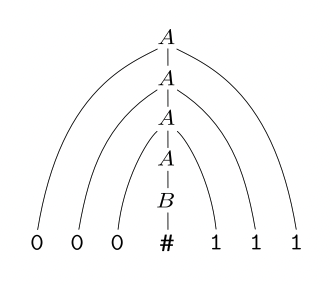
\includegraphics[width=\linewidth / 2]{lecture08-g1-parse-tree.png}

    Pulling all the leaves from the tree (shown by thin lines), we can see the string that is generated.
    Every word that is generated/derived from the start state has a parse tree.
    Grammars and parse tress come from linguistics. \\

    For example, English has a grammar and can be parsed.
\end{example}

\newpage
\subsection{Formal Definition Of A Context-Free Grammar}
\begin{definition}
    A \textbf{context-free grammar} is a 4-tuple $(V,\Sigma,R,S)$, where:
    \begin{itemize}
        \item $V$ is a finite set called the \textbf{variables}
        \item $\Sigma$ is a finite set, disjoint from $V$, called the \textbf{terminals}
        \item $R$ is a finite set of \textbf{rules}, with each rule being a variable and a string of variables and terminals, shown below
        $$\text{variable}\rightarrow\text{string}$$
        \item $S\in V$ is the start variable
    \end{itemize}
\end{definition}

If $u,v,w$ are strings of variables and terminals, and $A\rightarrow w$ is a rule of the grammar, we say that $uAv$ yields $uwv$, written $uAv\Rightarrow uwv$.
Say that $u\text{ derives } v$, written $u\Rightarrow v$, if $u=v$ or if a sequence $u_1,u_2,...,u_k$ exists for $k\geq 0$ and $$u\Rightarrow u_1\Rightarrow ...\Rightarrow u_k\Rightarrow v$$ \\


\begin{example}
    Consider the grammar $G_2=(\{S\},\{a,b\}R,S)$. The set of rules $R$ is $$S\rightarrow aSb\mid SS\mid\epsilon$$

    This grammar generates strings such as $abab$, $aaabbb$, and $aabaab$.
    Think of $a$ as '(' and $b$ as ')'. Viewed in this way, $L(G_3)$ is the language of all strings of properly nested (balanced) parentheses.
    Note that the language may contain the empty string $\epsilon$.
\end{example}

\begin{example}
    Consider the grammar $G_3=(V,\Sigma,R,\langle EXPR\rangle)$. \\

    $V$ is $\{\langle EXPR\rangle,\langle TERM\rangle,\langle FACTOR\rangle\}$ and $\Sigma$ is $\{a,+,\times, (, )\}$
    \begin{align*}
        \langle EXPR\rangle &\rightarrow\langle EXPR\rangle+\langle TERM\rangle\mid\langle TERM\rangle \\
        \langle TERM\rangle &\rightarrow\langle TERM\rangle\times\langle FACTOR\rangle\mid\langle FACTOR\rangle \\
        \langle FACTOR\rangle &\rightarrow (\langle EXPR\rangle)\mid a
    \end{align*}

    The two strings $a+a\times a$ and $(a+a)\times a$ are both generated with grammar $G_3$. The parse trees are shown below:

    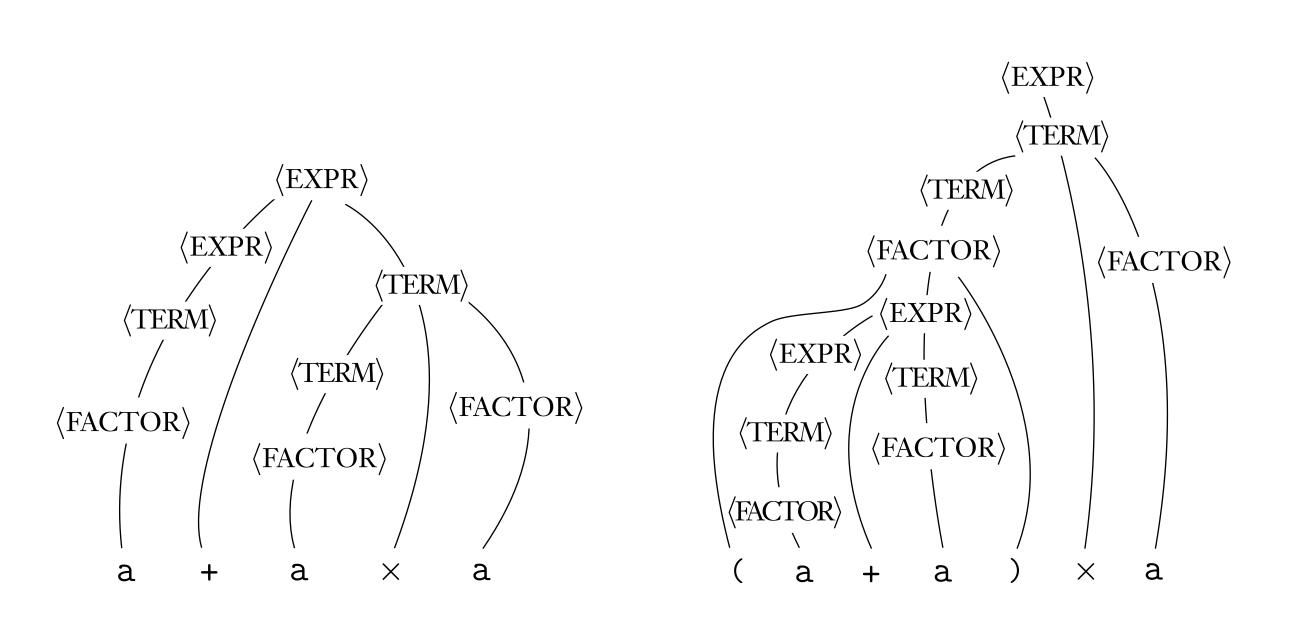
\includegraphics[width=\linewidth]{lecture08-g3-ex.png}
\end{example}

\subsection{Designing Context-Free Grammars}

Many CFLs are unions of simpler CFLs. \\

\begin{example}
    To get a grammar for the language $\{0^n1^n\mid n\geq 0\}\cup \{1^n0^n\mid n\geq 0\}$, first construct the grammar. \\

    $S_1\rightarrow 0S_1 1\mid\epsilon$ for language $\{0^n1^n\mid n\geq 0\}$
    $S_2\rightarrow1S_2 0\mid\epsilon$ for language $\{1^n0^n\mid n\geq 0\}$ \\

    Then add the rule $S\rightarrow S_1\mid S_2$ to give the grammar:
    \begin{align*}
        S &\rightarrow S_1\mid S_2 \\
        S_1 &\rightarrow 0S_1 1\mid\epsilon \\
        S_2 &\rightarrow 1S_2 0\mid\epsilon
    \end{align*}
\end{example}

Constructing a CFG for a language that happens to be regular is easy if you can first construct a DFA for that language.
You can convert any DFA into an equivalent CFG by:
\begin{enumerate}
    \item Make a variable $R_i$ for each state $q_i$ of the DFA.
    \item Add the rule $R_i\rightarrow aR_j$ to the CFG if $\delta(q_i,a)=q_j$ is the transition in the DFA.
    \item Add the rule $R_i\rightarrow\epsilon$ if $q_i$ is an accepting state of the DFA.
    \item Make $R_0$ the start variable of the grammar, where $q_0$ is the start state of the machine
\end{enumerate}

Certain CFLs contain strings with two substrings that are "linked" in the sense that a machine for such a language would need to remember an unbounded amount of information about one of the substrings to verify that it corresponds properly to the other substring. \\

\begin{example}
    Consider the language $\{0^n1^n\mid n\geq 0\}$. \\

    The machine would need to remember the number of 0s in order to verify that it equals the number of 1s.
    You can construct a CFG to handle this situation by using a rule of the form $R\rightarrow uRv$, which generates strings wherein the portion containing the $u$'s correspond to the portion containing the $v$'s.
\end{example}


In more complex languages, the strings may contain certain structures that appear recursively as part of other (or the same) structures.
An example is Example 3, where the grammar generates arithmetic expressions. Any time a symbol $a$ appears, an entire parenthesized expression might appear recursively instead.
To do this, put the variable symbol generating the structure in the location of the rules corresponding to where that structure may recursively appear.


\subsection{Nondeterminism With CFGs}
CFGs are in some sense nondeterministic because at each step, we can choose:
\begin{enumerate}
    \item which rule to apply
    \item which variable to apply the rule
\end{enumerate}

\begin{example}
    Consider the string $0AB1A0$. \\

    We can eliminate nondeterminism for (2) with leftmost derivation (applying the rule to the leftmost variable).
    However we cannot entirely eliminate nondeterminism because there can be multiple choices for the rule from a variable such as $A\rightarrow w_1\mid w_2\mid w_3\mid w_4$.
\end{example}

\subsection{Ambiguity}
If the grammar generates the same string in several ways, we say that the string is derived \textbf{ambiguously}.
If a grammar generates some string ambiguously, we say that the grammar is \textbf{ambiguous}. \\

More formally, if $w\in L(G)$, then $S\stackrel{*}{\Rightarrow}w$. Sometimes $S\stackrel{*}{\Rightarrow}w$ in more than 1 way, and if this happens with $G$, then $G$ is ambiguous. \\

\begin{example}
    Let $L=\{a^ib^jc^k\mid i=j\text{ or }j=k\}$. \\

    It can be shown that $L$ is generated by a CFG, and $L$ is inherently ambiguous. Consider the following grammar $G_5$ for $L$:
    \begin{align*}
        S & \rightarrow S_1C\mid AS_2 \\
        S_1 & \rightarrow aS_1b\mid\epsilon \\
        S_2 & \rightarrow bS_2c\mid\epsilon \\
        A & \rightarrow aA\mid\epsilon \\
        C & \rightarrow Cc\mid\epsilon \\
    \end{align*}

    A string such as $aabbcc$ can be generated through multiple different paths.
\end{example}

\begin{example}
    Consider grammar $G_4=(V,\Sigma,R,\langle EXPR\rangle)$.

    $$\langle EXPR\rangle\rightarrow \langle EXPR\rangle+\langle EXPR\rangle\mid\langle EXPR\rangle\times\langle EXPR\rangle\mid (\langle EXPR\rangle)\mid a$$

    The following is two parse trees for the string $a+a\times a$ in grammar $G_4$.

    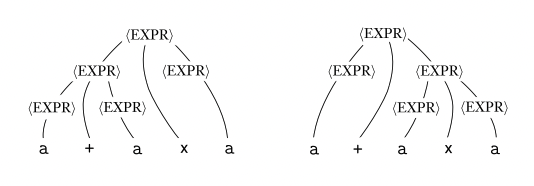
\includegraphics[width=\linewidth]{lecture08-g4-ex.png}

    Note that grammar $G_4$ does not capture the usual precedence relations ($\times$ before +).
\end{example}

\end{document}